\chapter{Chapter}
\thispagestyle{fancy} % Needed for Footer and Header on Chapterpage
\blindtext
\section{Section}
\blindtext
\subsection{Subsection}
\blindtext
\paragraph{Paragraph} \hfill \newline
\blindtext
\section{Aufzählung}
\subsection{Itemize}
\begin{itemize}
\item Das erste Item
Lorem ipsum dolor sit amet, consetetur sadipscing elitr, sed diam nonumy eirmod tempor invidunt ut labore et dolore magna aliquyam erat, sed diam voluptua. At vero eos et accusam et justo duo dolores et ea rebum. Stet clita kasd gubergren, no sea takimata sanctus est Lorem ipsum dolor sit amet. Lorem ipsum dolor sit amet, consetetur sadipscing elitr, sed diam nonumy eirmod tempor invidunt ut labore et dolore magna aliquyam erat, sed diam voluptua. At vero eos et accusam et justo duo dolores et ea rebum. Stet clita kasd gubergren, no sea takimata sanctus est Lorem ipsum dolor sit amet.
\item Das zweite Item
\begin{itemize}
\item Das erste Item
\item Das zweite Item
\item Das dritte Item
\end{itemize}
\item Das dritte Item
\end{itemize}

\subsection{Enumerate}
\begin{enumerate}
  \item The first item
  \item The second item
  \item The third etc \ldots
\end{enumerate}

\subsection{Description}
\begin{description}
  \item[First] The first item
  \item[Second] The second item
  \item[Third] The third etc \ldots
\end{description}
\begin{description}
  \item[First] \hfill \\
  The first item
  \item[Second] \hfill \\
  The second item
  \item[Third] \hfill \\
  The third etc \ldots
\end{description}

\section{Anführungszeichen}
Ich bin umfasst von \flqq Anführungszeichen \frqq{ }

\section{Links}
\url{https://www.wikibooks.org}
\href{https://www.wikibooks.org}{Wikibooks home}

\section{Footnote}
  Ich bin ein Footnotetest\footnote{\url{www.google.com}}



\section{Codesnippets}
\begin{lstlisting}
sudo apt-get install qemu
\end{lstlisting}

\section{Tabellen}

\begin{table}[htb]
\centering
    \begin{tabular}{@{} l l r@{}}\toprule
    {Stockwerk} & {Hostname} & {Anzahl Ports}\\ \midrule
    1 & DataCSW01 & 12\\ \addlinespace
    & DataCSW03 & 12\\ \addlinespace
    & DataCSW04 & 12\\ \addlinespace
    2& DataCSW02 & 24\\
    \bottomrule
    \end{tabular}
\caption{\textbf{Tabellen Unterschrift}}
\end{table}

\section{Bilder}
\begin{figure}[htbp]
	\begin{center}
	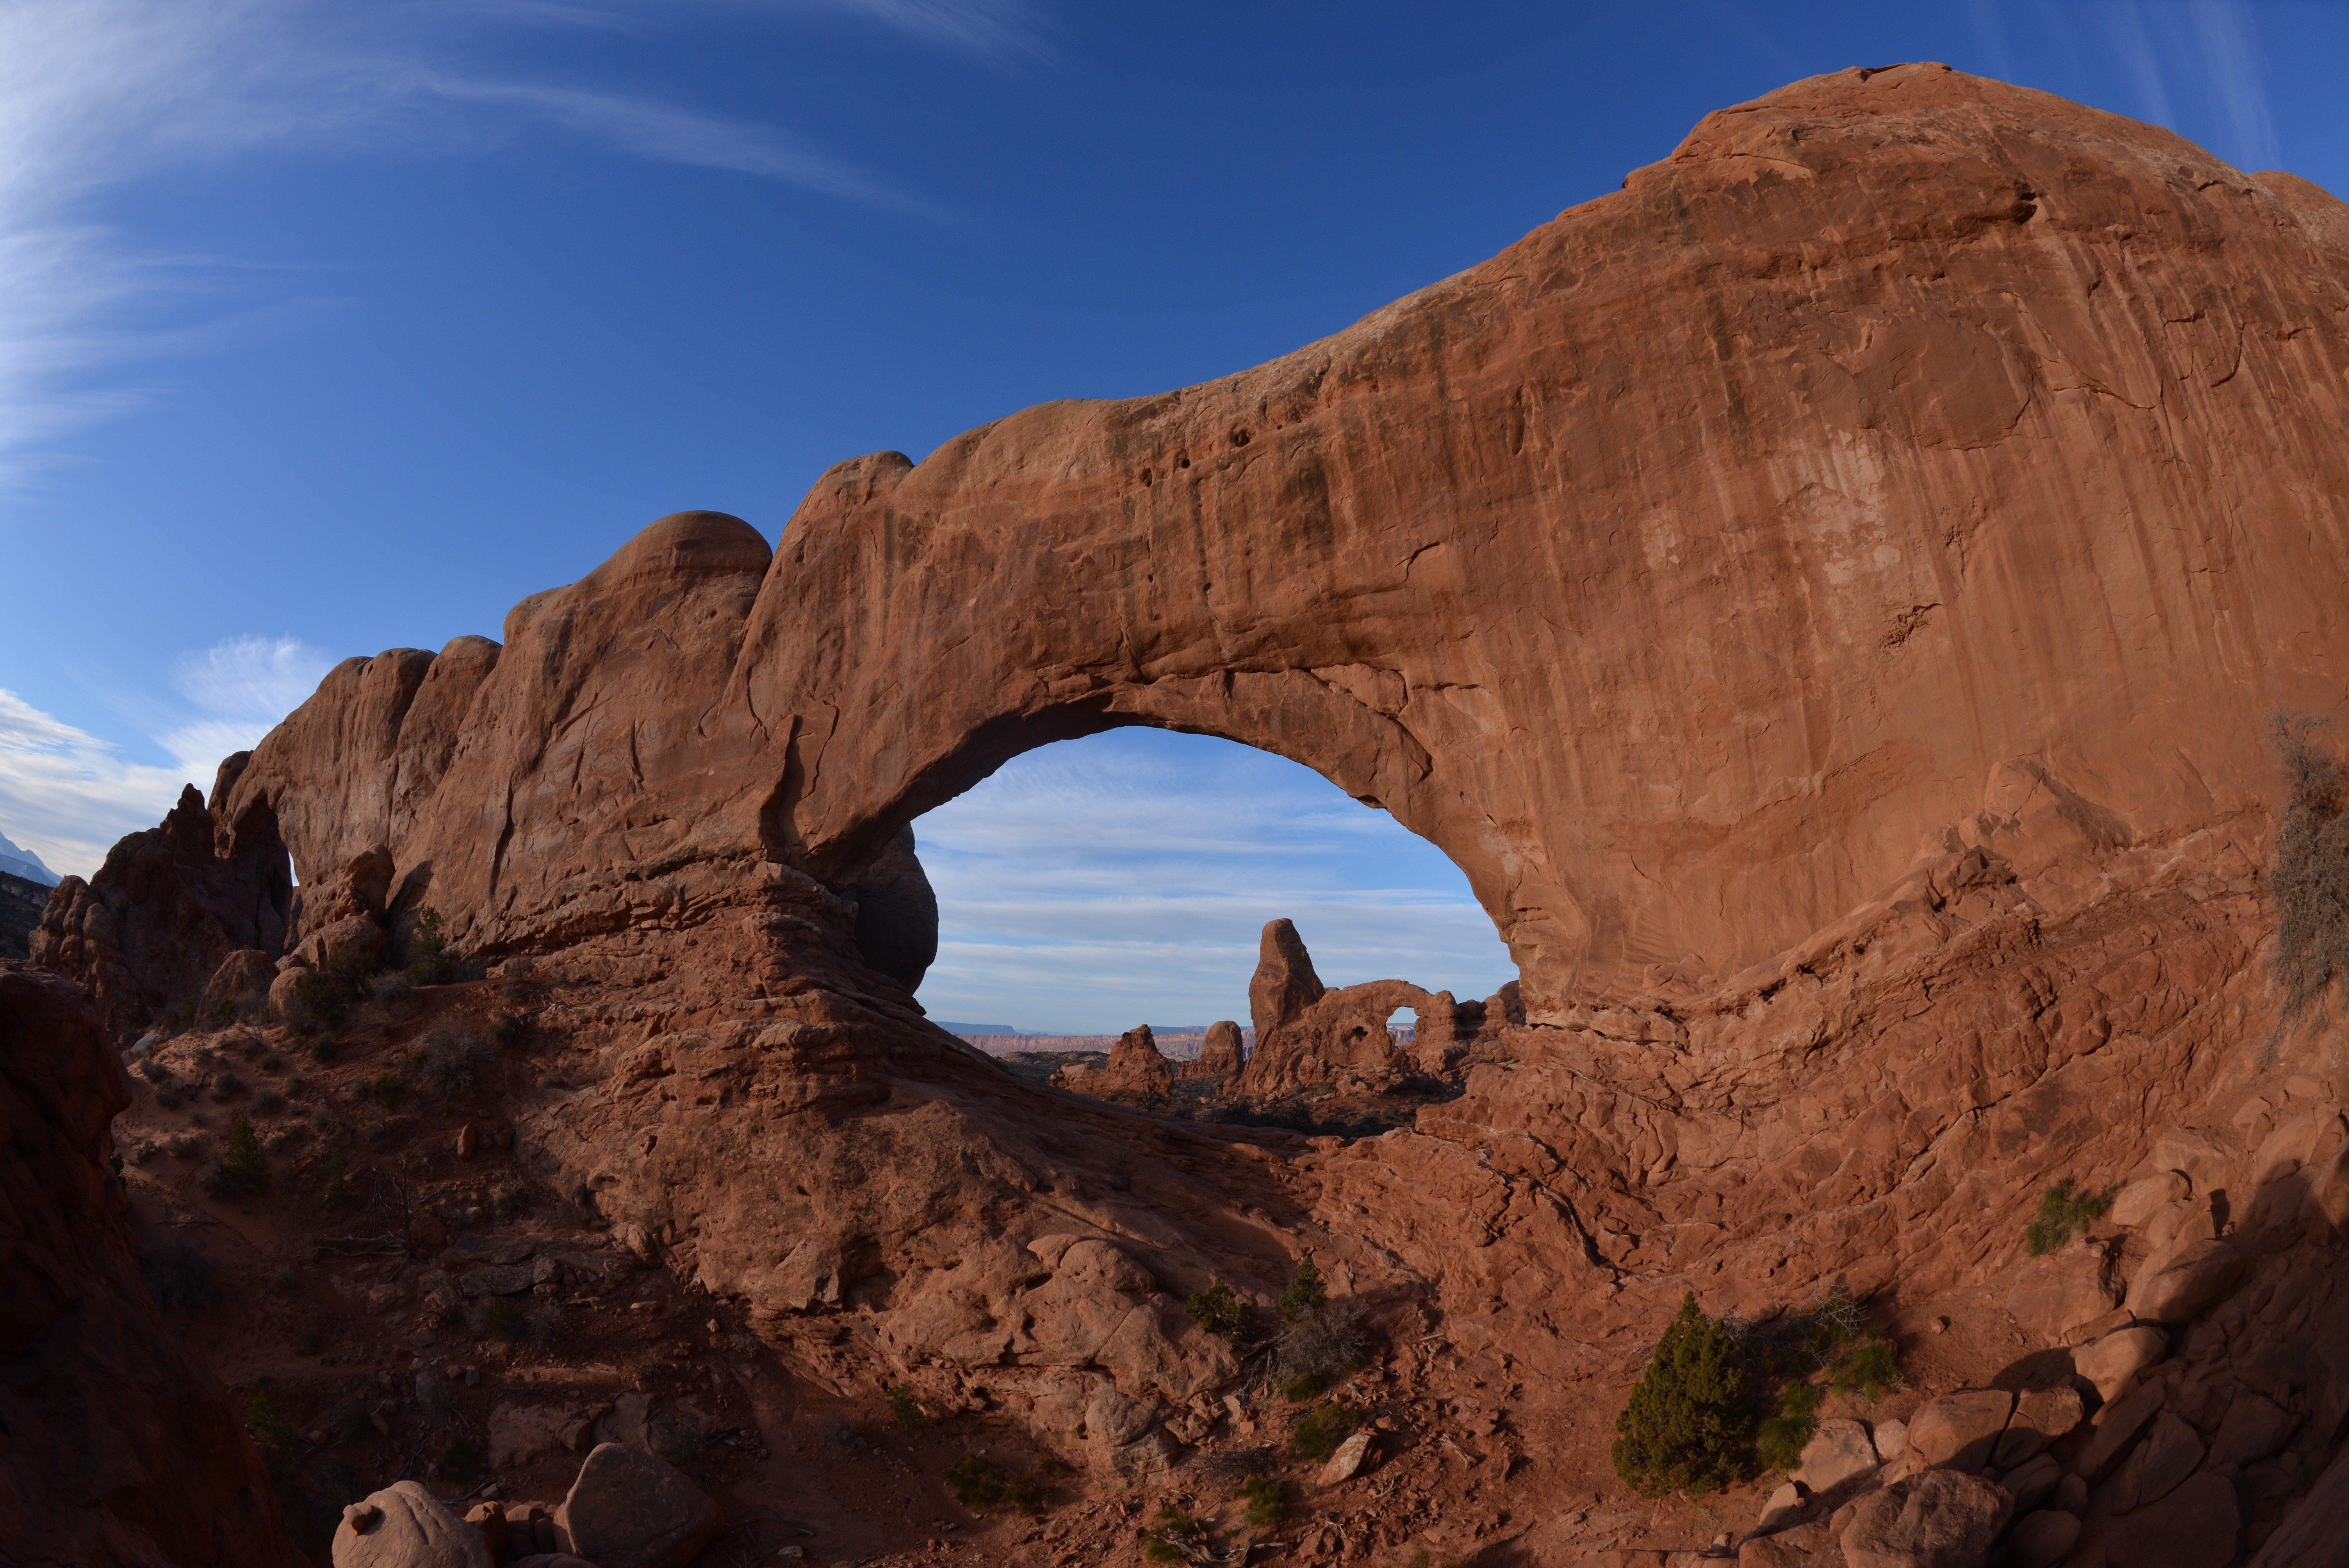
\includegraphics[width=0.50\textwidth]{./images/sampleImage.jpg}
	\caption{\textbf{Bild Unterschrift}}
	\label{Bild Referenz}
	\end{center}
\end{figure}

\begin{landscape}
\begin{figure}[htbp]
\subsection{Querformat}
\centering
\fbox{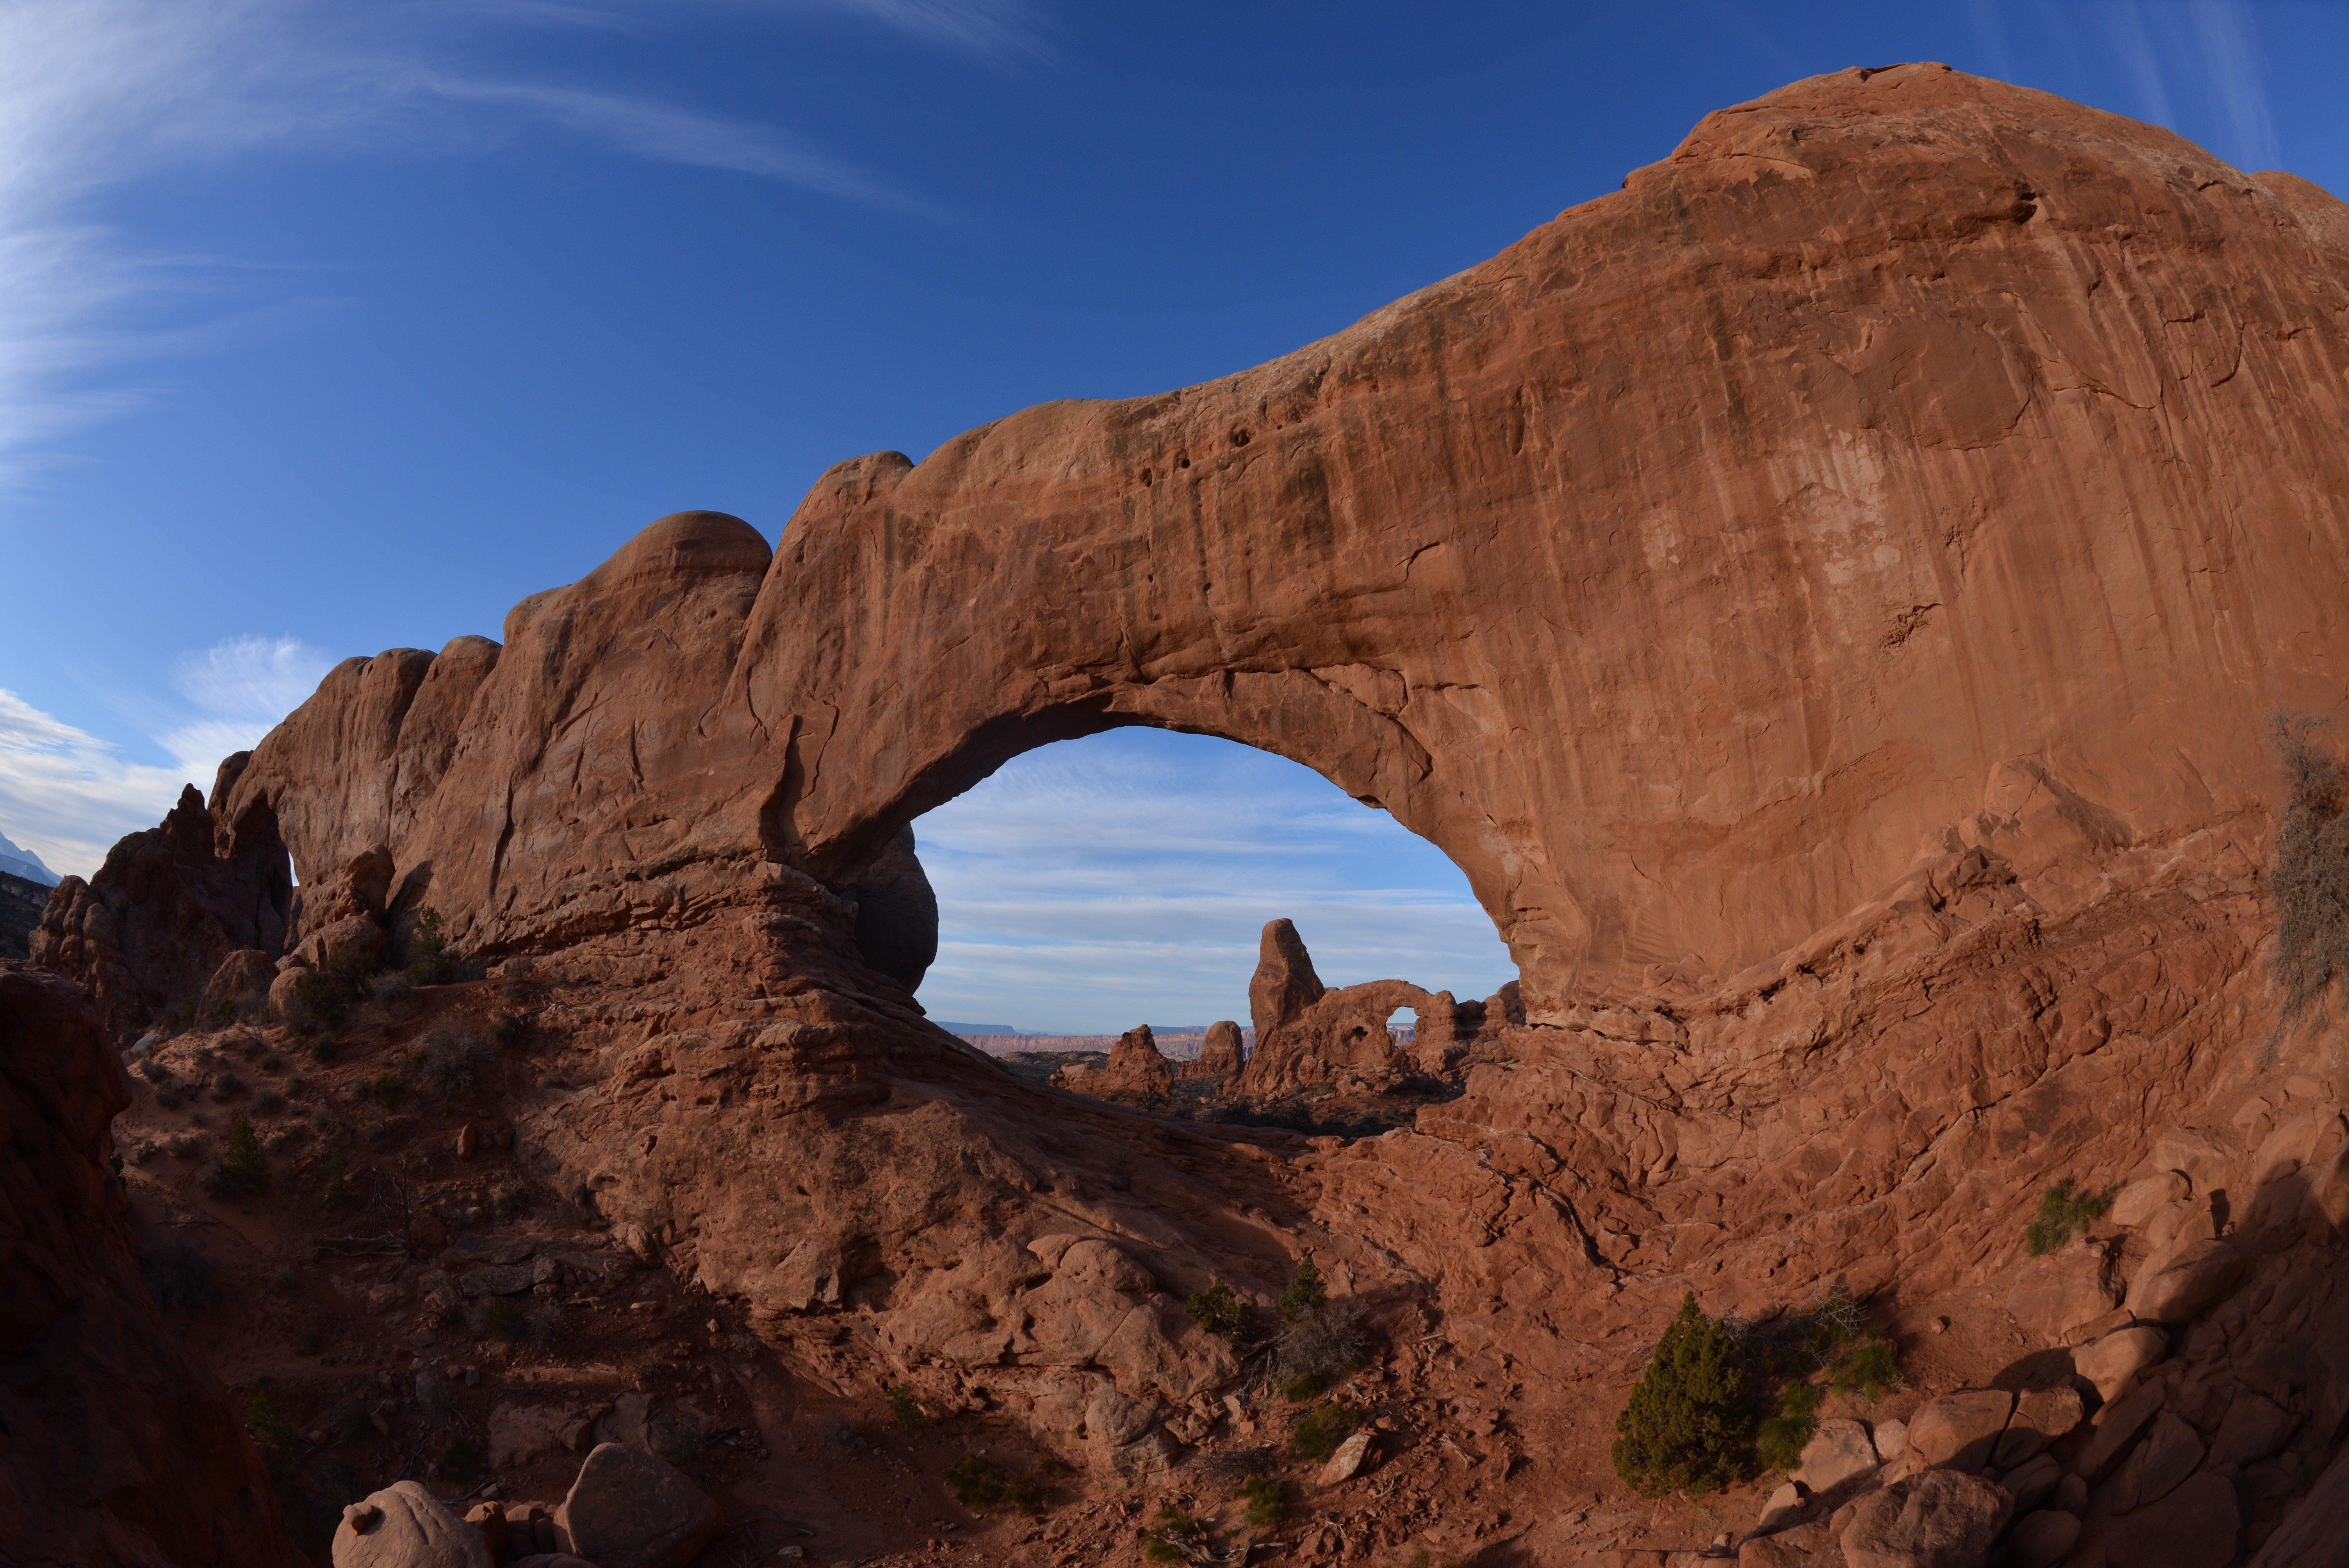
\includegraphics[width=\linewidth, height=\textheight,keepaspectratio]{./images/sampleImage.jpg}}
\caption{\textbf{Bild Querformat}}
\end{figure}
\end{landscape}

\section{Literaturverzeichnis}
Die Quellen sind in einem eigenen File ausgelagert wo sie definiert sind. Mittels \\cite{xxx} kann darauf verwiesen werden.


Ths document is an example of BibTeX using in bibliography management. Three items
are cited: \textit{The \LaTeX\ Companion} book \cite{latexcompanion}, the Einstein
journal paper \cite{einstein}, and the Donald Knuth's website \cite{knuthwebsite}.
The \LaTeX\ related items are \cite{latexcompanion,knuthwebsite}.

\section{Glossar und Akronyme}
Das Glossar ist in einem eigenen File ausgelagert wo es definiert ist.


The \Gls{latex} typesetting markup language is specially suitable
for documents that include \gls{maths}. \Glspl{formula} are
rendered properly an easily once one gets used to the commands.

Given a set of numbers, there are elementary methods to compute
its \acrlong{gcd}, which is abbreviated \acrshort{gcd}. This
process is similar to that used for the \acrfull{lcm}.
